% xjupiter-c3-server.tex

\documentclass{standalone}
% jupiter-illustration-preamble.tex

\usepackage{tikz}
\usetikzlibrary{shapes, positioning, arrows.meta, calc, backgrounds, fit}

\def\hdist{1.8}
\def\vdist{2.0}
\tikzset{node distance = \vdist and \hdist}

\tikzset{every lower node part/.style = {red}}
\newcommand{\statesplit}[4]{% #1: state upper label; #2: state lower label; #3: position; #4: name
  \node (#4) [circle split, draw, minimum size = 6mm, text width = 10mm, align = center, #3, font = \Large]
  {
    $#1$
    \nodepart{lower}
    $#2$
  };
}

\newcommand{\rectsplit}[2]{% #1: state upper label; #2: state lower label
  \node [draw, rectangle split, rectangle split parts = 2, 
    align = center, font = \Large]
  {
    #1
    \nodepart{two}
    \textcolor{red}{#2}
  };
}

\newcommand{\transition}[4][]{% #2: start state; #3: end state; #4: transition label; #1: transition label position (optional)
  \draw[>=Stealth, ->] (#2) to node (#2to#3) [rectangle, draw, above = 2pt, sloped, #1, font = \small] {$#4$} (#3);
}

\newcommand{\set}[1]{\{#1\}}
\newcommand{\ins}[2]{\textsc{Ins}(#1,#2)}
\newcommand{\del}[2]{\textsc{Del}(#2)}
% \newcommand{\del}[2]{\textsc{Del}(#1,#2)}


\newcommand{\digraph}[3]{% #1: name; #2: scale #3: style
  \node (#1) [#3] {\includegraphics[scale = #2]{xjupiter-c3-server-s2ss-#1}};
}

\begin{document}
\begin{tikzpicture}[node distance = 0.0cm and 1.1cm, 
  op/.style = {draw, rectangle},
  bg/.style = {rectangle, draw, inner sep = 0pt},
  size/.style = {scale = 0.40}]
  \digraph{c1-0}{0.3}{label = {above : ${\scriptstyle s2ss[c_1]}$}}
  \digraph{c2-0}{0.3}{right = 25pt of c1-0, label = {above : ${\scriptstyle s2ss[c_2]}$}}
  \digraph{c3-0}{0.3}{right = 35pt of c2-0, label = {above : ${\scriptstyle s2ss[c_3]}$}}
  \node (c30) [right = 1.8cm of c3-0, label = {above : ${\scriptstyle c2ss[c_3]}$}]
    {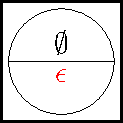
\includegraphics[scale = 0.3]{xjupiter-c3-0}};

  \digraph{c1-1}{0.25}{below = of c1-0}
  \digraph{c2-1}{0.25}{below = of c2-0}
  \digraph{c3-1}{0.25}{below = of c3-0, 
    label = {[yshift = -5pt, size] above : \fbox{$1: \ins{x}{1}$}}}
  \node (c31) [below = of c30, label = {[yshift = -5pt, size] above : \fbox{$1: \ins{x}{1}$}}] 
    {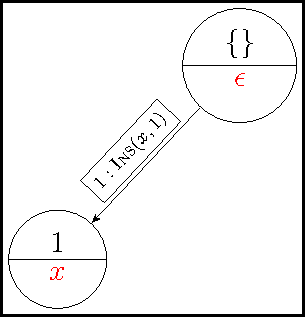
\includegraphics[scale = 0.25]{xjupiter-c3-1}};

  \digraph{c1-2}{0.2}{below = of c1-1}
  \digraph{c2-2}{0.2}{below = of c2-1}
  \digraph{c3-2}{0.2}{below = of c3-1,
    label = {[yshift = -5pt, size] above : \fbox{$2: \del{x}{1}$}}}
  \node (c32) [below = of c31, label = {[yshift = -5pt, size] above : \fbox{$4: \ins{b}{2}$}}] 
    {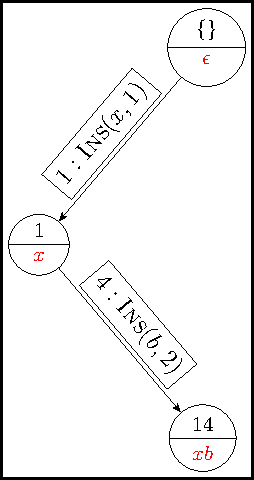
\includegraphics[scale = 0.2]{xjupiter-c3-2}};

  \digraph{c1-3}{0.2}{below = of c1-2}
  \digraph{c2-3}{0.2}{below = of c2-2}
  \digraph{c3-3}{0.2}{below = of c3-2,
    label = {[yshift = -5pt, size] above : \fbox{$3: \ins{a}{1}$}}}
  \node (c33) [below = of c32, label = {[yshift = -5pt, size] above : \fbox{$2: \del{x}{1}$}}] 
    {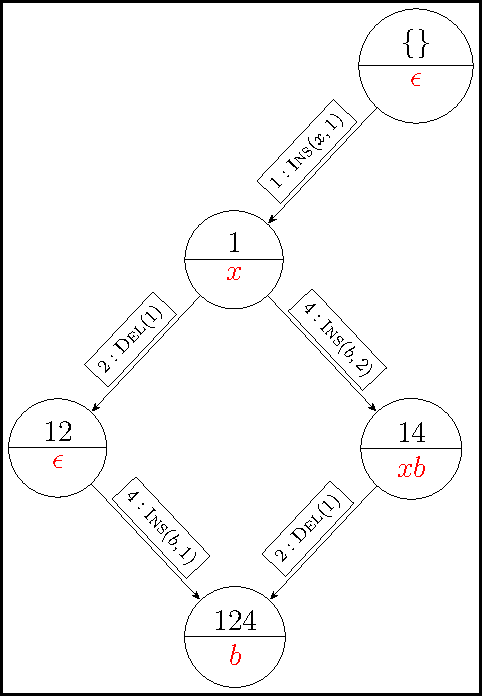
\includegraphics[scale = 0.2]{xjupiter-c3-3}};

  \digraph{c1-4}{0.2}{below = of c1-3}
  \digraph{c2-4}{0.2}{below = of c2-3}
  \digraph{c3-4}{0.2}{below = of c3-3,
    label = {[yshift = -5pt, size] above : \fbox{$4: \ins{b}{2}$}}}
  \node (c34) [below = of c33, label = {[yshift = -5pt, size] above : \fbox{$3: \ins{a}{1}$}}
  ] {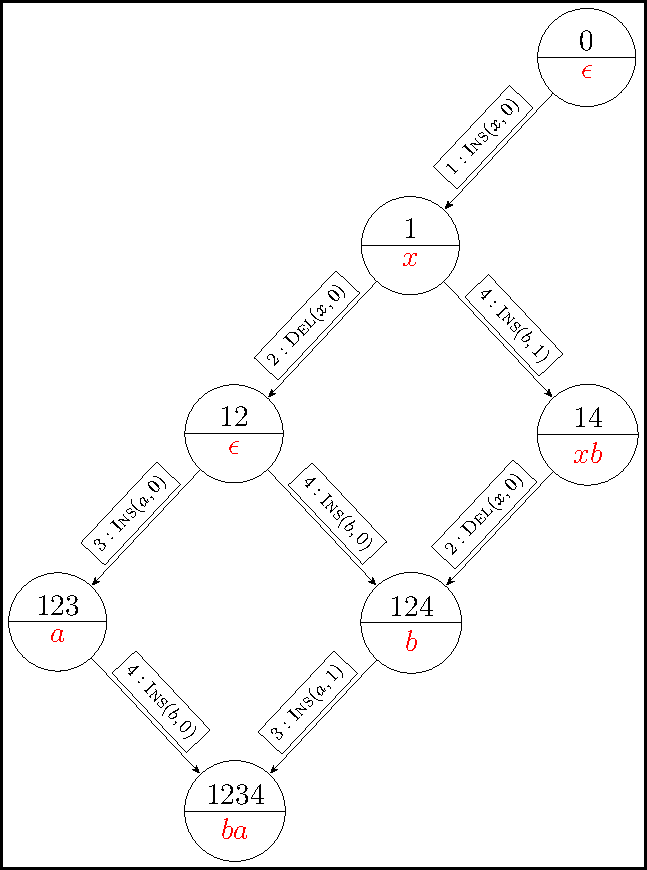
\includegraphics[scale = 0.2]{xjupiter-c3-4}};

  \node [bg, fit = (c1-0) (c1-4) (c3-0) (c3-4), label = {below : {\scriptsize Server}}] {};
  \node [bg, fit = (c30) (c34), label = {below : {\scriptsize Client} $c_3$}] {};
\end{tikzpicture}
\end{document}